\chapter{Dimensional Analysis}

\section{Introduction}
Dimensional analysis is a fundamental tool in understanding the relationships between different physical quantities.

\section{Classifications}

\begin{align*}
    \text{Circle:} \quad & (x-h)^2 + (y-k)^2 = r^2 \\
    \text{Sphere:} \quad & (x-h)^2 + (y-k)^2 + (z-l)^2 = r^2 \\
    \text{Disk:} \quad & (x-h)^2 + (y-k)^2 \leq r^2
\end{align*}
Here we ask: How many dimensions are needed to visualize these objects? The answer depends on the number of variables in the equation.

\begin{itemize}
    \item{\textbf{Plane Lines:} 2 variables, 1 equation}
    \item{\textbf{Space Lines:} 3 variables, 2 equations}
\end{itemize}
Examples of planes:
\[
\text{xy-plane : } z = 0
\]
\[
\text{xz-plane : } y = 0
\]
\[
\text{yz-plane : } x = 0
\]
Examples of lines:
\[
\text{x-axis : }
\begin{cases}
    z = 0\\
    y = 0
\end{cases}
\]
\[
\text{y-axis : }
\begin{cases}
    x = 0\\
    z = 0
\end{cases}
\]
\[
\text{z-axis : }
\begin{cases}
    x = 0\\
    y = 0
\end{cases}
\]
\pagebreak
\section{Geometric Equations}

\subsection{Distance Between Two Points}

The distance \(d_{PQ}\) between two points \( P(x_1, y_1, z_1) \) and \( Q(x_2, y_2, z_2) \) in three-dimensional space is given by:
\begin{equation}\label{Distance Between Two Points}
    d_{PQ} = \sqrt{(x_2 - x_1)^2 + (y_2 - y_1)^2 + (z_2 - z_1)^2}
\end{equation}

\subsection{Distance Between a Point and a Plane}
\begin{equation} \label{Distance Between a Point and a Plane}
    \text{dist}(P, \Pi) = \dfrac{|\vec{P} \cdot \vec{n}|}{||\vec{n}||}
\end{equation}

\subsection{Distance Between Two Parallel Lines}
\begin{equation} \label{Distance Between Two Parallel Lines}
    \text{dist}(L_1, L_2) = \dfrac{|\vec{v_1} \cdot \vec{v_2}|}{||\vec{v_1}||}
\end{equation}

\subsection{Distance Between a Point and a Line}
\begin{equation} \label{Distance Between a Point and a Line}
    \text{dist}(P, L) = \dfrac{|\vec{P} \times \vec{v}|}{||\vec{v}||}
\end{equation}

\subsection{Midpoint Formula}

The midpoint \(M_{PQ}\) between two points \( P(x_1, y_1, z_1) \) and \( Q(x_2, y_2, z_2) \) is calculated as:
\begin{equation}\label{Midpoint Formula}
    M_{PQ} = \left(\dfrac{x_1 + x_2}{2}, \dfrac{y_1 + y_2}{2}, \dfrac{z_1 + z_2}{2}\right)
\end{equation}

\subsection{Equation of a Sphere}

A sphere centered at \(P(p, q, s)\) with radius \( r \) has the equation:
\begin{equation}\label{Equation of a Sphere}
    (x - p)^2 + (y - q)^2 + (z - s)^2 = r^2
\end{equation}

\subsection{Equation of a Circle}
\begin{equation}\label{Equation of a Circle}
    (x-h)^2 + (y-k)^2 = r^2
\end{equation}

\subsection{General Quadratic Equation with two unknowns}
\begin{equation}\label{General Quadratic Equation}
    Ax^2 + By^2 + Cxy + Dx + Ey + F = 0
\end{equation}
\[
    A^2 + B^2 + C^2 \neq 0, \quad A, B, C, D, E, F \in \R
\]
\subsection{Equation of an Ellipsoid}

An ellipsoid centered at \(P(h, k, l)\) is given by:

\begin{equation}\label{Equation of an Ellipsoid}
    \dfrac{(x-h)^2}{a^2} +  
    \dfrac{(y-k)^2}{b^2} + 
    \dfrac{(z-l)^2}{c^2} = 1
\end{equation}

\subsection{Equation of an Ellipse}
\begin{equation}\label{Equation of an Ellipse}
    \dfrac{(x-h)^2}{a^2} + \dfrac{(y-k)^2}{b^2} = 1
\end{equation}

\subsection{Equation of a Hyperbola}
\begin{equation}\label{Equation of a Hyperbola}
    \dfrac{(x-h)^2}{a^2} - \dfrac{(y-k)^2}{b^2} = 1
\end{equation}
\subsection{Equation of a Parabola}
\begin{equation}\label{Equation of a Parabola}
    (y-k)^2 = 4p(x-h)
\end{equation}

\subsection{Equations of a Line}
\(\vec{a_l} = \langle a, b, c \rangle\) is the vector collinear to the line, and \(P(x_0, y_0, z_0)\) is a point on the line.
\subsubsection{Parametric Form}
\begin{equation}\label{Parametric Form of a Line}
    l = 
    \begin{cases}
        x = x_0 + at\\
        y = y_0 + bt\\
        z = z_0 + ct
    \end{cases}
\end{equation}

\subsubsection{Normal Form}
\begin{equation}\label{Normal Form of a Line}
    \dfrac{x-x_0}{a} = \dfrac{y-y_0}{b} = \dfrac{z-z_0}{c}
\end{equation}

\subsection{Equations of a Plane}
\(\vec{a_l} = \langle a, b, c \rangle\) is the vector normal to the plane, and \(P(x_0, y_0, z_0)\) is a point on the plane.
\subsubsection{Point-Normal/Scalar Form}
\begin{equation}\label{Point-Normal Form of a Plane}
    a(x-x_0) + b(y-y_0) + c(z-z_0) = 0
\end{equation}

\section{Quadric Surfaces}

\subsection{Ellipsoid}
\begin{equation}\label{Equation of an Ellipsoid}
    \dfrac{x^2}{a^2} + \dfrac{y^2}{b^2} + \dfrac{z^2}{c^2} = 1
\end{equation}

\subsection{Hyperboloid of One Sheet}
\begin{equation}\label{Equation of a Hyperboloid of One Sheet}
    \dfrac{x^2}{a^2} + \dfrac{y^2}{b^2} - \dfrac{z^2}{c^2} = 1
\end{equation}

\subsection{Hyperboloid of Two Sheets}
\begin{equation}\label{Equation of a Hyperboloid of Two Sheets}
    -\dfrac{x^2}{a^2} - \dfrac{y^2}{b^2} + \dfrac{z^2}{c^2} = 1
\end{equation}

\subsection{Elliptic Cone}
\begin{equation}\label{Equation of an Elliptic Cone}
    \dfrac{x^2}{a^2} + \dfrac{y^2}{b^2} - \dfrac{z^2}{c^2} = 0
\end{equation}

\subsection{Elliptic Paraboloid}
\begin{equation}\label{Equation of an Elliptic Paraboloid}
    \dfrac{x^2}{a^2} + \dfrac{y^2}{b^2} = z
\end{equation}

\subsection{Hyperbolic Paraboloid}
\begin{equation}\label{Equation of a Hyperbolic Paraboloid}
    \dfrac{x^2}{a^2} - \dfrac{y^2}{b^2} = z
\end{equation}

\subsection{Describing Quadric Surfaces}
To describe a quadric surface, you need to know the cross sections of the surface with the coordinate planes. For example, the cross sections of an ellipsoid with the coordinate planes are ellipses.
\subsubsection{Example}
Given the equation \(x^2 + 4y^2 + 9z^2 = 36\), the cross sections with the coordinate planes are:
\begin{itemize}
    \item{\(z = 0\): Ellipse with major axis 6 and minor axis 2 given by the equation:}
    \[
        x^2 + 4y^2 = 36-9z^2
    \]
    \item{\(y = 0\): Ellipse with major axis 6 and minor axis 3 given by the equation:}
    \[
        x^2 + 9z^2 = 36-4y^2
    \]
    \item{\(x = 0\): Ellipse with major axis 4 and minor axis 3}
    \[
        4y^2 + 9z^2 = 36-x^2
    \]
\end{itemize}
Since all cross sections are ellipses, the surface is an ellipsoid.

Description: This is an ellipsoid centered at the origin with semi-axes of length 6, 3, and 2 along the x, y, and z-axes, respectively.

\section{Graphing Concepts}

Graphing helps visualize functions and equations by showing the set of all points that satisfy them.

\subsection{Functions of a Single Variable}

For a function of a single variable \( f(x) \):
\begin{itemize}
    \item \textbf{Domain}: A subset or all of the real number line, often denoted as \(\mathbb{R}\) or a specific interval such as \((- \infty, \infty)\).
    \item \textbf{Range}: The set of possible values of \( f(x) \); for instance, \([0, \infty)\).
    \item \textbf{Graph}: A curve on the Cartesian plane, representing ordered pairs \((x, f(x))\).
\end{itemize}

\subsection{Functions of Multiple Variables}

For functions of two or more variables, the domain and range extend to higher dimensions:
\begin{itemize}
    \item \textbf{Domain}: The set of all points in \(\mathbb{R}^n\) (e.g., \(\mathbb{R}^2\) for a function of two variables or \(\mathbb{R}^3\) for three variables) where the function is defined.\\
        - \textbf{Entire Plane}: If the function \( f(x, y) \) is defined for all \((x, y) \in \mathbb{R}^2\).\\
        - \textbf{Portion of the Plane}: A subset of \(\mathbb{R}^2\), specified by conditions like \(x > 0\) or \(y \geq 1\) or given by a picture.
    \item \textbf{Range}: The set of output values of the function. For many functions of multiple variables, this is a subset of \(\mathbb{R}\).
    \item \textbf{Graph}: For a function \( f(x, y) \) in two variables, the graph is a surface in three-dimensional space. For functions of three variables, the graph would exist in four-dimensional space and cannot be directly visualized.
\end{itemize}

\subsection*{Examples of Functions of Multiple Variables}

\textbf{1: Linear Function of Two Variables}
    \[
    f(x, y) = 3x + 5y - 7
    \]
    \begin{itemize}
        \item \textbf{Domain}: \(\mathbb{R}^2\) (all real pairs \((x, y)\))
        \item \textbf{Range}: \(\mathbb{R}\) (all real values)
        \item \textbf{Graph}: A plane in three-dimensional space.
    \end{itemize}

\textbf{2: Linear Function of Three Variables}
    \[
    f(x, y, z) = 3x - 5y + z - 11
    \]
    \begin{itemize}
        \item \textbf{Domain}: \(\mathbb{R}^3\) (all real triples \((x, y, z)\))
        \item \textbf{Range}: \(\mathbb{R}\)
        \item \textbf{Graph}: Exists in four-dimensional space; it cannot be visualized in three dimensions.
    \end{itemize}
\textbf{3: Rational Function of Two Variables}
    \[
        f(x, y) = 5 - 7 \sqrt{13-x^2-y^2-2x}
    \]
    \begin{itemize}
        \item \textbf{Domain}: $(x-1)^2+y^2 \leq 14$, disk with center $(1, 0)$ with radius $\sqrt{14}$.
        \begin{center}
            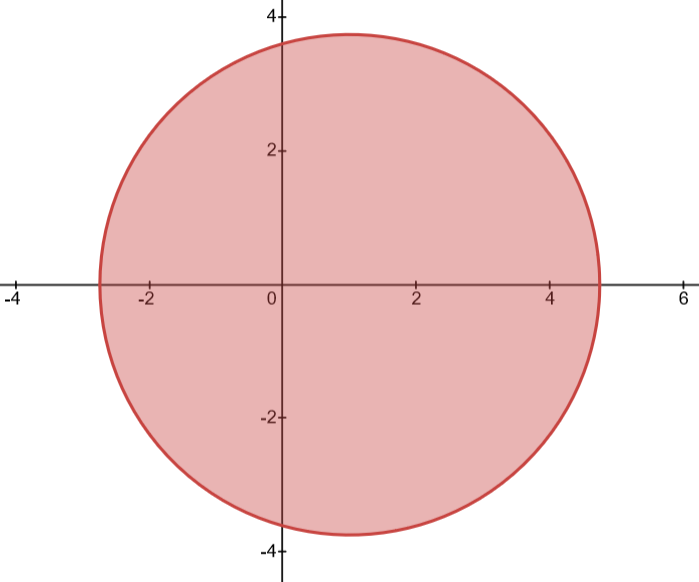
\includegraphics[width=0.3\textwidth]{domain1.png}
        \end{center}
        \item \textbf{Range}: $\left[5-7\sqrt{13}, 5\right]$
        \item \textbf{Graph}: A surface in three-dimensional space. This equation can be rewritten as 
        \[
            \dfrac{\left(x-1\right)^{2}}{14}+\dfrac{\left(y\right)^{2}}{14}+\dfrac{\left(z-5\right)^{2}}{49\cdot14}=1
        \] 
        \begin{center}
            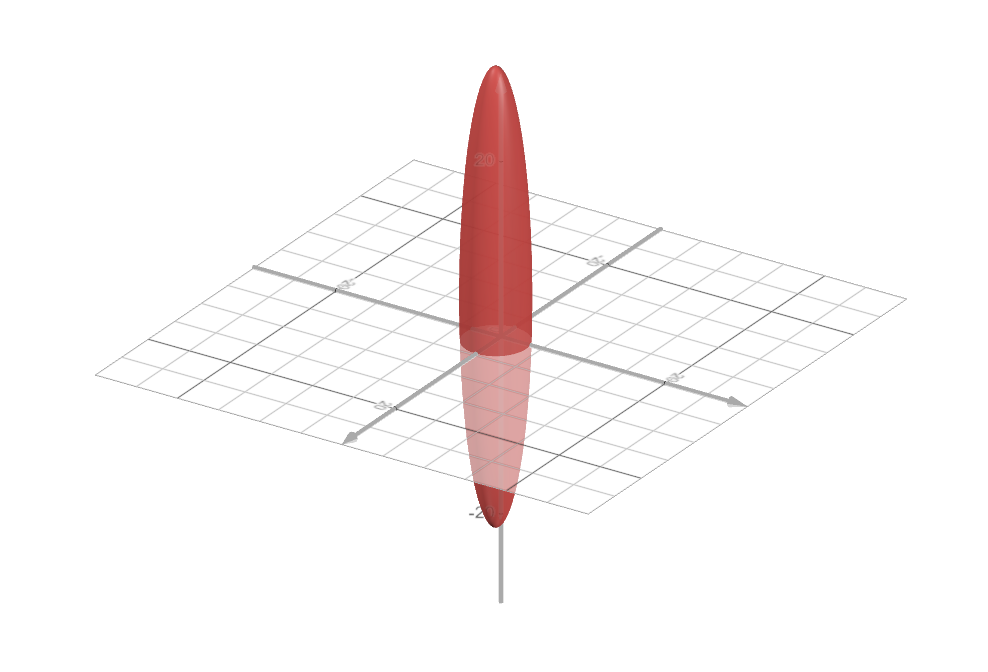
\includegraphics[width=0.5\textwidth]{graph1.png}
        \end{center}
    \end{itemize}

\textbf{4: Trigonometric Function of Two Variables}
    \[
        f(x,y) = 
        3 - \dfrac{5}{\pi}\arcsin(x+y)
    \]
    \begin{itemize}
        \item \textbf{Domain}: $-1 \leq x+y \leq 1$
        \begin{center}
            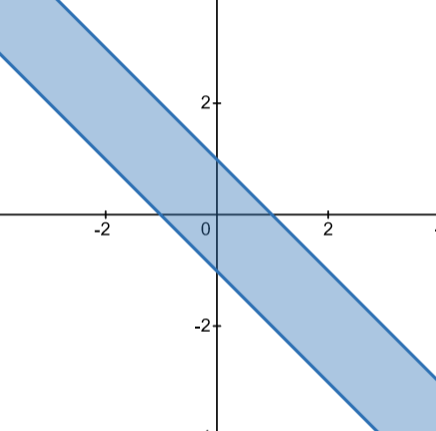
\includegraphics[width=0.3\textwidth]{domain2.png}
        \end{center}
        \item \textbf{Range}: \[\dfrac{-\pi}{2} \leq \arcsin(x+y) \leq \dfrac{\pi}{2}, \, z \in \left[\dfrac{1}{2}, \dfrac{11}{2}\right]\]
        \item \textbf{Graph}: A surface in three-dimensional space.
        \begin{center}
            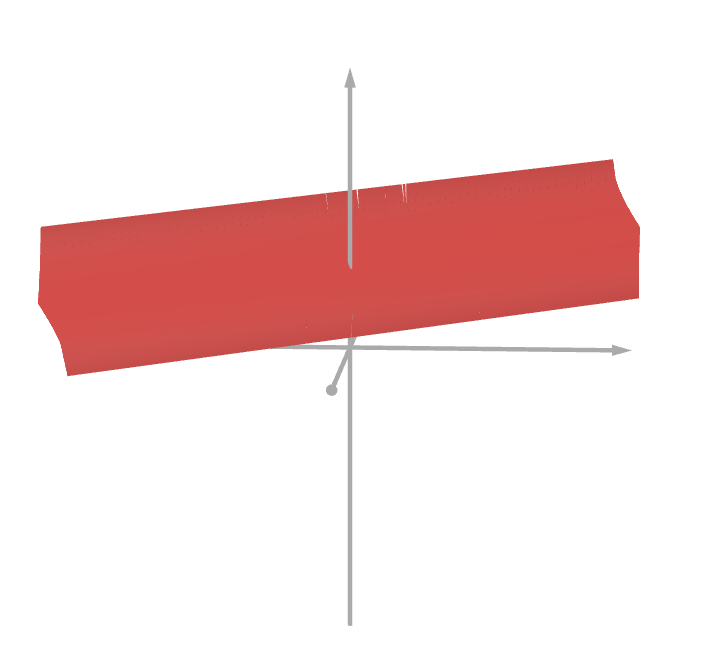
\includegraphics[width=0.5\textwidth]{graph2.png}
        \end{center}
    \end{itemize}
\section{Graphing Dimensions Summary}

Graphing dimensions change based on the variables involved:
\begin{itemize}
    \item \textbf{1D}: Interval or union of intervals
    \item \textbf{2D}: Picture
    \item \textbf{3D}: Description
    \item \textbf{4D and Higher}: Equation
\end{itemize}